\apendice{Documentación técnica de programación}

\section{Introducción}

En este apéndice voy a tratar de explicar todos los detalles técnicos necesarios para que las personas que desean trabajar con este proyecto o incluso continuarlo puedan hacerlo de manera sencilla.

\section{Estructura de directorios}

La siguiente estructura de directorios es la utilizada para la realización del proyecto y se puede encontrar en el siguiente repositorio \url{https://github.com/MJ0T4/Simulador_Domotica_Raspberry}.

\begin{itemize}
	\item \textbf{'/':} directorio raíz del proyecto. En el se encuentra el fichero \textit{README.md} y los siguientes directorios:
	\begin{itemize}
		\item \textbf{apk:} contiene la apk para realizar la instalación de la aplicación
		\item \textbf{app android:} contiene todo el proyecto referente a la parte de \textit{Android} con Android Studio.
		\begin{itemize}
			\item \textbf{app:} contiene el código fuente del proyecto.
			\begin{itemize}
				\item \textbf{src:} contiene el código fuente del proyecto.
				\begin{enumerate}
					\item \textbf{androidTest/java/mario/app android:} contiene los test instrumentales.
					\item \textbf{main}: contiene todas las clases java y todos los recursos del proyecto.
					\item \textbf{test/java/mario/app android:} contiene los test unitarios.
				\end{enumerate}
			\end{itemize}
		\end{itemize}
		\item \textbf{diseño:} contiene el archivo \textit{diseño.mdj} que contiene a su vez todos los diagramas realizado para este proyecto.
		\item \textbf{doc:} contiene la documentación del proyecto.
		\begin{itemize}
			\item \textbf{img:} contiene todas las imágenes utilizadas para la documentación de la memoria y anexos.
			\item \textbf{tex:} contiene cada uno de los ficheros correspondientes a la memoria y anexos.
		\end{itemize}
		\item \textbf{servidor raspberry:} contiene todo el proyecto referente a la parte de \textit{Python 3} con Jetbrains PyCharms.
		\begin{itemize}
			\item \textbf{imagenes:} contiene todas la imágenes utilizadas por la interfaz.
		\end{itemize}
	\end{itemize}
\end{itemize}

\section{Manual del programador}

En este apartado voy a hacer una breve explicación técnica del funcionamiento del proyecto.

\subsection{Raspberry Pi}

En la Raspberry Pi ejecutaremos el código desarrollado en Python 3. Dentro del directorio del proyecto de Python tenemos dos ficheros fundamentales.

\begin{itemize}
	\item El fichero \verb|Servidor.py| contiene toda la lógica de la interfaz y el servidor.
	\item El fichero \verb|Database.py| contiene todos los métodos que permiten realizar cambios en la base de datos.
\end{itemize}

Dentro del fichero \verb|Servidor.py| solo se encuentra una clase que controla todo. Dentro de ella existen métodos para la creación de la interfaz y su tratamiento y métodos para la inicialización del servidor y el tratamiento de mensajes. El hilo de ejecución de ambos se realiza a la vez en la llamada a la clase, pero cada uno tiene su hilo independiente.

\subsection{Aplicación Android}\label{sec:explicacionAndroid}

En este apartado sobre hablaré brevemente sobre los ficheros .java que se encuentran en el directorio \textbf{Simulador Domotica Raspberry/app android/app/src/main/java/mario/app android}. Dentro de este directorio nos encontramos con los siguientes ficheros.

\begin{itemize}
	\item \verb|BDLocal.java|: interfaz creada para declarar, pero no implementar, los métodos que se usarán para realizar cambios en la base de datos.
	\item \verb|BDSqlite.java|: implementa la interfaz \verb|BDLocal.java| y desarrolla los métodos declarados por ella.
	\item \verb|Conexion.java|: implementa una tarea asíncrona para mandar cambios al servidor.
	\item \verb|CustomAdapterEstancia.java|: adaptador personalizado para representar las filas de estancias en una \textit{ListView}.
	\item \verb|CustomAdapterLuz.java|: adaptador personalizado para representar las filas de bombillas en una \textit{ListView}.
	\item \verb|Habitacion.java|: implementa los elementos que irán en cada fila del adaptador \verb|CustomAdapterEstancia.java|.
	\item \verb|Home.java|: implementa la ventana principal donde se representarán las estancias de nuestra vivienda.
	\item \verb|Luz.java|: implementa los elementos que irán en cada fila del adaptador \verb|CustomAdapterLuz.java|.
	\item \verb|PlantillaLuces.java|: implementa la \textit{Activity} en la que se mostrarán las bombillas de una estancia.
	\item \verb|RecepcionSocket.java|: implementa la escucha de mensajes del servidor en un \verb|Thread| implementado la interfaz \verb|Runnable|.
	\item \verb|Servidor.java|: implementa la modificación de datos del servidor, su conexión y desconexión.
\end{itemize}

\section{Compilación, instalación y ejecución del proyecto}

Para comenzar con la compilación del proyecto es necesario descargarlo a través de \textit{GitHub} \url{https://github.com/MJ0T4/Simulador_Domotica_Raspberry}. Una vez tenemos el proyecto descomprimido comenzamos a trabajar con él.

Para realizar la compilación del proyecto Android, tendremos que instalar previamente la herramienta de desarrollo \textbf{Android Studio}. Para ello, podemos descargar el ejecutable desde el siguiente enlace:

\url{https://developer.android.com/studio/}

Una vez descargado e instalado, lo ejecutamos. Dentro de la ventana principal nos digirimos al menú superior de opciones. En el seguiremos los siguientes pasos:
\begin{enumerate}
	\item Pulsar sobre la opción \verb|File| del menú de opciones.
	\item Pulsar sobre la opción \verb|New| del menú que se ha desplegado.
	\item Pulsar sobre la opción \verb|Import project| del menú que se ha desplegado nuevamente.
	\item Se abrirá un explorador de archivos en el que debemos buscar el directorio \verb|app_android| del proyecto que hemos descargado.
	\item Una vez seleccionado lo cargamos y ya tendremos el proyecto en nuestro Android Studio.
\end{enumerate}

Con el proyecto ya cargado en la herramienta Android Studio solo debemos pulsar sobre el icono de un martillo verde y el proyecto comenzará a compilarse.

\begin{figure}[h!]
	\centering
	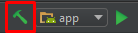
\includegraphics[width=0.4\linewidth]{img/martillo}
	\caption{Icono para la compilación del proyecto.}
	\label{fig:martillo}
\end{figure}

La ejecución del proyecto es posible realizarla sobre un emulador virtual de Android que viene incluido con la herramienta o sobre un terminal físico. Para la ejecución mediante el emulador virtual solo debemos pulsar sobre el botón con símbolo \textit{Play} de color verde que se puede ver en la imagen \ref{fig:martillo}. Si por el contrario deseamos realizar la instalación de la apk debemos mirar la sección \ref{sec:instalacionAndroid}. Para conocer los posibilidades que tiene esta aplicación tanto en el emulador virtual como en el terminal físico mirar la sección \ref{sec:manualAndroid}.

La compilación del proyecto de la parte de Raspberry Pi no es necesaria ya que simplemente con la ejecución del fichero \verb|Servidor.py| se realiza la compilación. Para realizar la instalación del proyecto de Python en la Raspberry Pi mirar la sección \ref{sec:instalacionRaspberry}. Y para su ejecución y funcionamiento mirar la sección \ref{sec:ejecuciónRaspberry}.

\section{Pruebas del sistema}

Durante la realización de este proyecto, las pruebas sobretodo de la parte de Android han sido realizadas manualmente a través de un emulador de Android que proporciona la herramienta Android Studio. Solo existía una parte del proyecto que no se podía visualizar y era la parte de la base de datos. Por ello, creí conveniente realizar un test instrumental que comprobase el correcto funcionamiento de los métodos de la base de datos sobre el emulador virtual de Android.\\
En la parte de la Raspberry Pi, las pruebas también se han realizado manualmente, además de que su código no es muy extenso. Para comprobar el correcto funcionamiento de la base de datos, como en la parte de Android, he utilizado el programa \textit{DB Browser for Sqlite}. A través de este programa he podido visualizar las tablas y el contenido del archivo \textit{database}. Este programa se puede descargar desde el siguiente repositorio:

\url{https://github.com/sqlitebrowser/sqlitebrowser/releases}